\chapter{Versuch}
Beim Versuch wurde das Leiter bzw. Halbleiterplättchen jeweils in ein homgenes Magnetfeld gestellt. Die Stärke des Magnetfeldes wurde mit einem Teslameter bestimmt. An das Hallplätchen wurde ein Querstrom $I_Q$ angelegt und varriiert. Es wurde die Hallspannung $U_H$ in Abhängigkeit zum Querstrom gemessen.

Anhand der Messwerte wurde jeweils
\begin{itemize}
\item die Hallkonstante $R_H$
\item die Ladungsträgerkonzentration $n$
\item die Driftgechwindigkeit der Ladungsträger $v$
\end{itemize}
bestimmt.

Beim Silberplättchen wurde zusätzlich noch die Anzahl der Leitungselektronen pro Atom bestimmt.

\section{Silberplättchen}

\subsection{Material}
\begin{itemize}
\item Silberplättchen
\item Labornetzteil für den Querstrom (bis \SI{20}{\ampere})
\item 2 Spulen als Vorwiderstand für das Silberplättchen
\item Elektromagnet
\item Labornetzteil für den Elektromagneten (bis \SI{5}{\ampere})
\item Mobile-CASSY mit Mikrovoltbox
\item Hochstromzange
\item Teslameter
\end{itemize}

\subsection{Durchführung}
Das Silberplättchen wurde in den Elektromagneten eingespannt.
Die beiden Spulen des Elektromagneten wurden in Reihe geschaltet und an ein Labornetzteil angeschlossen.
Die beiden Anschlüsse des Silberplättchens wurden an ein weiteres Labornetzteil angeschlossen. Die beiden Spulen wurden in Reihe geschaltet und ebenfalls in Reihe in den Querstromkreis eigebaut.
Die beiden Anschlüsse für die Hallspannung am Silberplättchens wurden an die Mikrovoltbox angeschlossen, welche an das Mobile-Cassy gesteckt wurde.

Dann wird der Elektromagnet eingeschaltet. Der Strom betrug $I_{mag} = \SI{4.74}{\ampere}$
Das Teslameter wurde außerhalb des Magnetfeldes justiert, so dass es \SI{0}{\milli\tesla} anzeigt.
Dann wurde die Sonde senkrecht zur Feldrichtung in das Magnetfeld des Elektromagneten gehalten.

Der Elektromagnet wurde wieder ausgeschaltet. Dann wurde der Querstrom eingeschaltet und auf den niedrigsten möglichen Wert, $I_Q = \SI{3}{\ampere}$ eingestellt. Das Potentiometer am Plättchen wurde so eingestellt, dass die gemessene Hallspannung mit ausgeschaltetem Magnetfeld \SI{0}{\milli\volt} betrug. Mit der Stromzange wurde die Querstromstärke bestimmt. Dazu wurde sie um eines der Kabel, durch dass der Querstrom fließt gelegt. Der Elektromagnet wurde eingeschaltet und die gemessene Hallspannung mit der Querstromstärke notiert. Dieser Vorgang wurde dann in \SI{1}{\ampere}-Schritten bis \SI{20}{\ampere} wiederholt.

\subsection{Messergebnisse}
Für das Silberplättchen erhielten wir bei einem Magnetfeld mit $B = \SI{195}{\milli\tesla}$. Das Plättchen hat eine Dicke von $d = \SI{5e-5}{\meter}$

\begin{figure}[H]
\centering
\csvreader[tabular=cc, table head=Querstrom $I_Q$ in \SI{}{\ampere} & Hallspannung $U_H$ in \SI{}{\micro\volt}\\\Xhline{4\arrayrulewidth}, late after line=\\\hline]{data/silber.dat}{}{\num{\csvcoli} & \num{\csvcolii}}
\caption{Messwerte mit Silber}
\end{figure}

Für eine Fehlerrechnung werden folgende Fehler zu Grunde gelegt:
\begin{align*}
I_Q &: \pm \SI{0.5}{\ampere} \\
U_H &: \pm \SI{1}{\micro\volt} \\
B &: \pm \SI{6}{\milli\tesla} \\
\end{align*}

\begin{figure}[H]
\centering
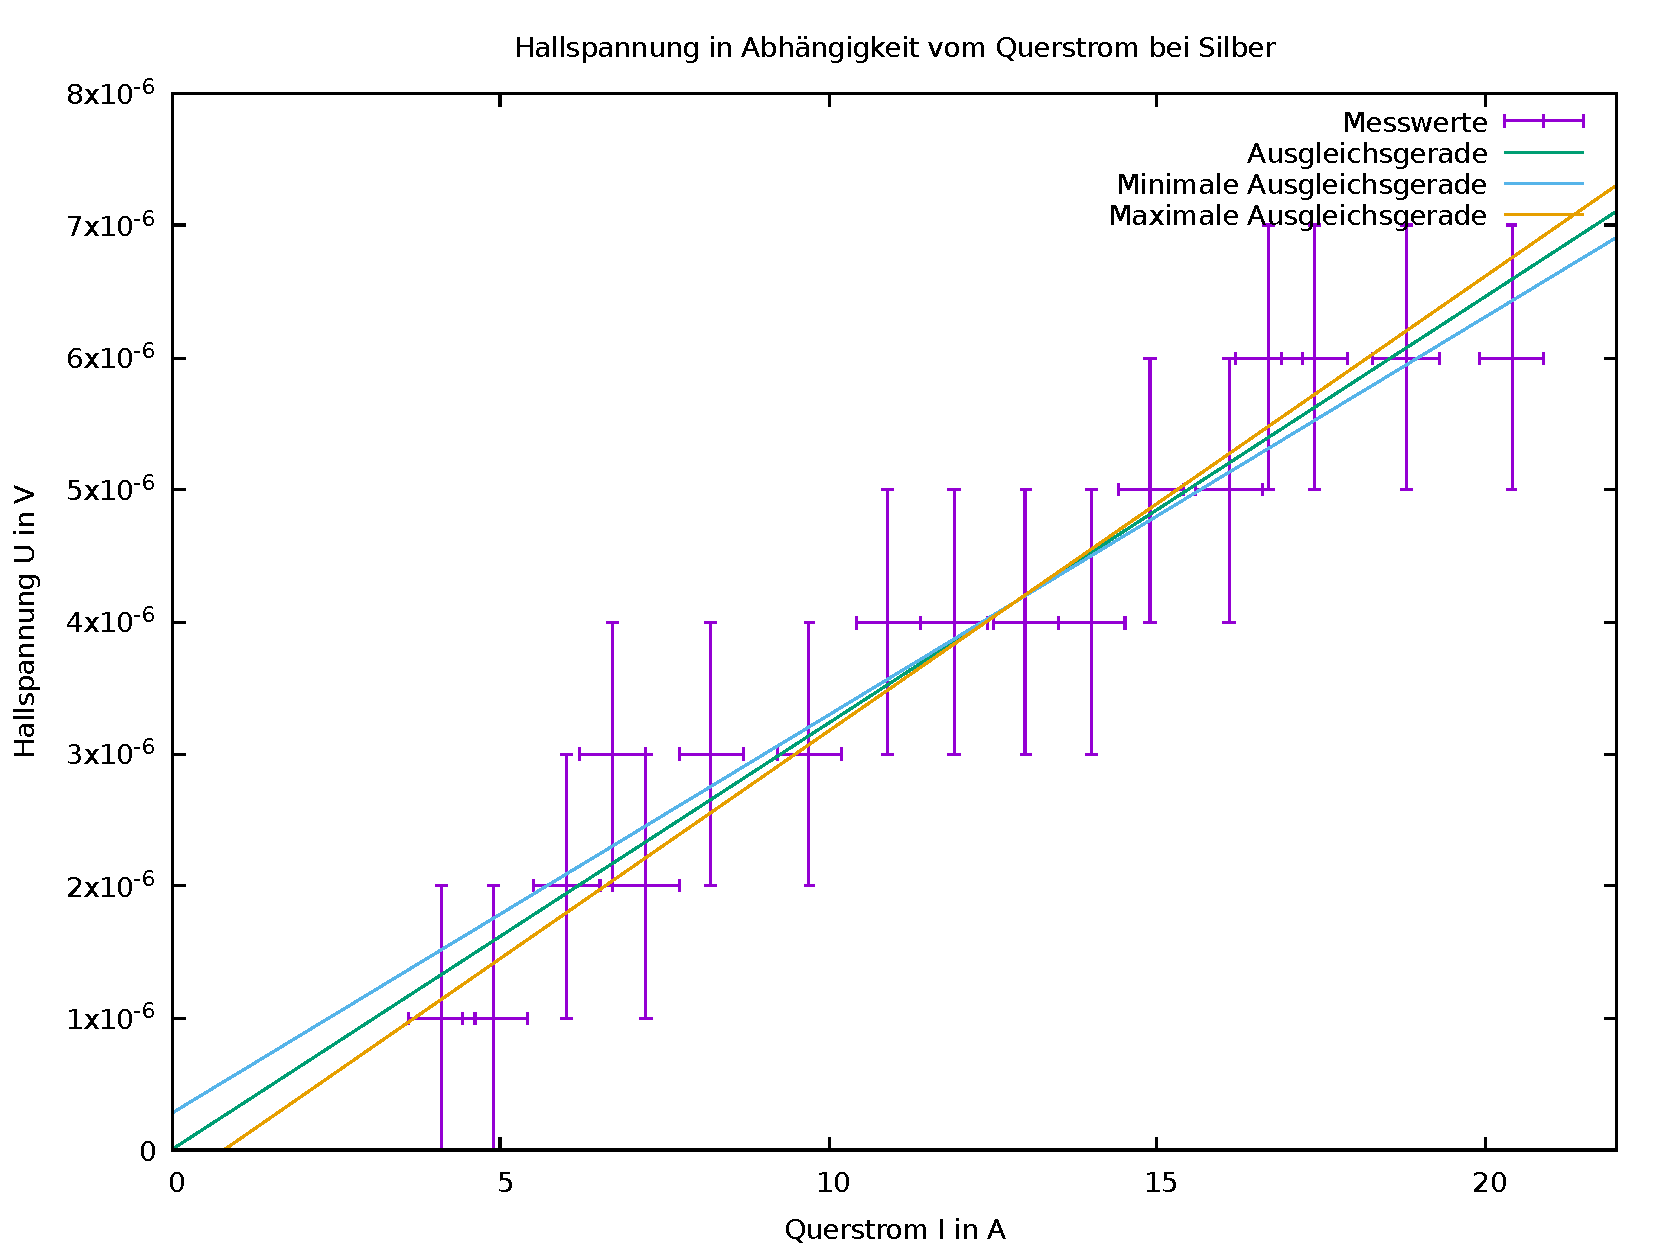
\includegraphics[width=\textwidth]{data/silber.pdf}
\caption{Graphische Darstellung und Auswertung der Messwerte mit Silber}
\end{figure}

\subsection{Auswertung}
Mit \texttt{GNUplot} wurde eine lineare Regression durchgeführt. Für die Steigung der Geraden erhält man
$$m = \SI{3.226 \pm 0.214e-7}{\volt\per\ampere}$$


\subsubsection{Hallkonstante}

Für die Hallspannung gilt folgende Formel:
$$U_H = \frac{B \cdot I_Q}{d} \cdot \frac{1}{n \cdot e}$$

Der rechte Teil $\frac{1}{n \cdot e}$ ist die Hallkonstante $R_H$.
$$R_H = \frac{U_H}{I_Q \cdot B}$$

Aus der Steigung kann man $R_H$ so bestimmen:
\begin{align*}
m &= \frac{U_H}{I_Q} \\
R_H &= \frac{m \cdot d}{B}
\end{align*}

Für unsere Messwerte ergibt das:
\begin{align*}
R_H &= \frac{\SI{3.226 \pm 0.214e-7}{\volt\per\ampere} \cdot \SI{5e-5}{\meter}}{\SI{195 \pm 6}{\milli\tesla}} \\
R_H &= \SI{8.27}{\cubic\meter\per\coulomb}
\end{align*}

Der Fehler beträgt:
\begin{align*}
\Delta R_H &= \SI{8.27e-11}{\cubic\meter\per\coulomb} \cdot \sqrt{\left(\frac{\SI{0.214e-7}{\volt\per\ampere}}{\SI{3.226e-7}{\volt\per\ampere}}\right)^2 + \left(\frac{\SI{6e-3}{\tesla}}{\SI{195e-3}{\tesla}}\right)^2} \\
&= \SI{6.05e-12}{\cubic\meter\per\coulomb}
\end{align*}
Somit kann man die Hallkonstante für das Silberplättchen angeben
$$R_H = \SI{8.27 \pm 0.61e-11}{\cubic\meter\per\coulomb}$$
Laut Anleitung beträgt die Hallkonstante \SI{8.9e-11}{\cubic\meter\per\coulomb}.
Der Literaturwert liegt somit knapp außerhalb des Fehlerbereichs.

\subsubsection{Ladungsträgerkonzentration}
Die Ladungsträgerkonzentration kann man aus der bereits ermittelten Hallkonstante bestimmen.
\begin{align*}
R_H &= \frac{1}{n \cdot e} \\
n &= \frac{1}{R_H \cdot e} \\
  &= \frac{1}{\SI{8.27e-11}{\cubic\meter\per\coulomb} \cdot \SI{1.602e-19}{\coulomb}} \\
  &= \SI{7.55e28}{\per\cubic\meter}
\end{align*}

Für den Fehler:
\begin{align*}
\Delta n &= \SI{7.55e28}{\per\cubic\meter} \cdot \frac{\SI{0.61e-11}{\cubic\meter\per\coulomb}}{\SI{8.27e-11}{\cubic\meter\per\coulomb}} \\
&= \SI{0.56e28}{\per\cubic\meter}
\end{align*}

Die Ladungsträgerkonzentration kann mit
$$n = \SI{7.55 \pm 0.56e28}{\per\cubic\meter}$$
angegeben werden.

\subsubsection{Anzahl der Leitungselektronen pro Atom}
Die Dichte von Silber beträgt
$$\rho_{Ag} = \SI{10490}{\kilo\gram\per\cubic\meter}$$
Die Molare Masse von Silber beträgt
$$M_{Ag} = \SI{0.1079}{\kilo\gram\per\mole}$$
\begin{align*}
m_{Ag} &= \rho_{Ag} \cdot V \\
N_{Ag} &= \frac{m_{Ag}}{M_{Ag}} \cdot N_A & \text{Zahl der Silberatome}\\
z &= \frac{n \cdot V}{N_{Ag}} & \text{Ladungsträger pro Atom}\\
  &= \frac{n \cdot M_{Ag}}{\rho_{Ag} \cdot N_A} \\
  &= \frac{\SI{7.55e28}{\per\cubic\meter} \cdot \SI{0.1079}{\kilo\gram\per\mole}}{\SI{10490}{\kilo\gram\per\cubic\meter} \cdot \SI{6.022e23}{\per\mole}} \\
  &= 1.28
\end{align*}

Der Fehler beträgt:

\begin{align*}
\Delta z &= 1.28 \cdot \frac{\SI{0.56e28}{\per\cubic\meter}}{\SI{7.55e28}{\per\cubic\meter}}\\
&\approx 0.09
\end{align*}
Somit kann man das Verhältnis aus Ladungsträgern und Atomen angeben mit:
$$z = \SI{1.28 \pm 0.09}{}$$

\subsubsection{Driftgechwindigkeit}
